\documentclass[11pt]{article}
\usepackage{acl2014}
\usepackage{times}
\usepackage{url}
\usepackage{latexsym}


%\documentclass[twocolumn]{article}
%\usepackage[margin=2cm,a4paper]{geometry}

\usepackage{amsmath}
\usepackage{subcaption,graphicx}
\usepackage{enumerate}
\usepackage{hyperref}


\usepackage{tikz}
\tikzset{
    embedding/.style={rectangle,draw=black,text centered},
    index/.style={circle,draw=black,text centered, text width=0.45cm},
    hidden/.style={rectangle split,rectangle split horizontal=true,rectangle split parts=7,draw=black},
}
\usetikzlibrary{shapes}
\usetikzlibrary{positioning,backgrounds}

\title{Multilingual Word Embeddings from Sentence Representations}
\author{Benno Kruit\\10576223\\benno.kruit@student.uva.nl\And
Sara Veldhoen\\10545298\\sara.veldhoen@student.uva.nl}
\date{\today}
\begin{document}
\maketitle


\begin{abstract}

By representing the meaning of language in a vector space, we can model many semantic phenomena in a natural way.
These representations have also proven useful for many Natural Language Processing tasks.
We propose a method for using multilingual sentence embeddings to construct word embeddings in a shared vector space.
We also highlight the difference between approaches that rely on local word context and on co-occurrence within sentences.
Our model learns word embeddings that share features across multiple languages.
We evaluate our word embeddings on a cross-lingual document classification task on multiple corpora.


\end{abstract}

\section{Introduction}\label{s:introduction}

%% Role of alignments & window %%


%% Topic vs function vectors %% 



%% Usefulness of joint multilingual embeddings and evaluation %% 

% Given only sentence alignments, 



Distributional semantics is a fast developing field that concerns the establishment of a semantic vector space were words have a geometrical interpretation. We investigate how to use data in multiple languages to create a single multilingual semantic space. The word representations in this vector space may have a theoretical interest on their own right, but can also be used for tasks related to translation, such as cross-lingual information retrieval and machine translation. 

We introduce an approach to induce such cross-lingual word embeddings using sentence-aligned data, based on sentence co-occurrence. We show how this is fundamentally different from approaches that focus on local co-occurrence in an n-gram context. Without word alignments, local co-occurrence cannot be used in cross-lingual induction of word embeddings. Global (sentence-based) co-occurrence yields word embeddings that are less informative of the function of a word in a sentence, but can be quite useful in Information Retrieval tasks. We use such a task to evaluate the quality of our embeddings, namely cross-lingual document classification.

This document is structured as follows. In section~\ref{relatedWork}, we discuss several  approaches to multilingual distributional semantics. We introduce two existing monolingual models to obtain sentence embeddings in section~\ref{s:sentenceEmbeddings}, and extend them for the multilingual case. We explain how word embeddings can be obtained in section~\ref{s:wordEmbeddings}. The tasks we use for evaluation of the resulting embeddings are described in section~\ref{s:evaluation}, followed by the experiments we conducted and emperical results in section~\ref{s:experiments}. In section~\ref{s:discussion}, we set forth some considerations and ideas for future investigation of this topic. We conclude with some final remarks in section~\ref{s:conclusion}.


\section{Related Work}\label{s:relatedWork}
Some research has focused on the induction of multilingual word embeddings, using both different techniques to obtain word representations, and different approaches to the cross-lingual aspects. The evaluation methods applied also vary a lot.


\subsection{Linear Mapping}\label{s:lin}
% Using a dictionary

According to Mikolov et al. \cite{mikolov2013exploiting}, the vector space of word representations in different languages are geometrically similar, because words in languages are grounded in real world concepts.
It is therefore possible to find a linear mapping 
%(rotation and scaling) 
between these vector spaces.

The approach is to first train word embeddings on large monolingual data for both languages separately, using the \texttt{word2vec} implementation. In the reported experiments, the so-called CBOW architecture is used, that predicts a word given its context in both directions.
% Notably, the authors also propose a way to include some phrases: multi-word expressions. This may prove useful for translation, as one multiple words can together express a concept that has a single word in another language.

Using a relatively small set of gold standard word translations, in this case obtained from Google Translate, a transformation matrix $W$ is searched. The training objective is to minimize the distance between words that are translations of one another.

The evaluation is performed on a test set of gold-standard word translations, again from Google Translate. The word representation in the source language is transformed using $W$, and a ranked list of the nearest words in the target language is the output. The precision at ranks 1 and 5 is reported.

% Not parallel data, but simple dictionary (Google Translate) used as gold standard. Because of this, every word has one single gold-standard translation, instead of a similarity score to several words
% Easy evaluation method = nice
% Maybe the assumption of linear translation is too strong. The interrelation of some concepts may be evident for strong real-world concepts such as cat and dog, but some concepts may be more culturally determined: friendship, politics. Also, Asian cultures have a very different understanding of time. What about nonlinear mappings: e.g. stretching some bit of the space, and shrinking another bit?

\subsection{Multitask Learning}
% Using alignments

Klementiev and Titov \cite{klementiev2012inducing} induce distributed representations for a pair of languages jointly. By doing so, words in both languages are represented in a single vector space.

The induction is treated as a multitask learning problem where each task corresponds to a single word. The training influences other tasks depending on the task-relatedness. The latter is derived from co-occurrence statistics in bilingual parallel data: the number of alignment links between  that word and its (supposed) translations. 

The word representations are induced in a neural language model architecture. 
The $n$ preceding words form the context, their representations are concatenated to form a context vector. The probability of the next word occuring is predicted from this vector. The training procedure aims to find the word representations that minimize the data (log) likelihood: 
$L(\theta) = \sum_{t=1}^T \log \hat{P}_\theta (w_t|w_{t-n+1:t-1})$. 

The method is evaluated on a real-world task: crosslingual document classification. Topic annotations are available for documents in one of the languages, and the system predicts the topics of documents in the other language. The jointly induced word representation outperform two other approaches to the problem: glossing (where every word in the document is translated separately, based on word alignments) and Machine Translation.


\subsection{Joint Learning from Sentence Embeddings}
% No alignment, but compositionality

Unlike the previous approaches, Hermann and Blunsum \cite{hermann2013multilingual} start from sentence alignments, which share the same semantics.
The assumption is that some function can describe the composition of word embeddings into a sentence embedding.
For the sake of their argument, the authors use a simple bag-of-words additive interpretation of composition. 
The word embeddings are induced jointly for both languages from these sentence-embeddings, by minimizing the distance between both sums of word embeddings.
% However, the sentence embeddings are not present a priori, nor is the training aimed at obtaining these.
% ? the sentence embeddings are not learned? 
% Nope, just the fact that two sentences should have the same semantics is used.
In order to make sure the weights won't be reduced to zero, similarity between unaligned sentence embeddings is penalized.
%This method is implemented in a software package named \texttt{bicvm}.

The same evaluation as in \cite{klementiev2012inducing} is applied, i.e. the document classification task. Furthermore, the authors present a graphical qualitative analysis. 
In \cite{Hermann2014}, this approach is expanded by evaluating on a larger number of language pairs.

\subsection{An Autoencoder Approach}
% No alignment, no compositionality

Recent work that is highly relevant constructs word embeddings using a sentence autoencoder \cite{SarathChandar2014autoencoder}.
The autoencoder predicts which words are in a sentence given the (transformed) sum of their embeddings.
Building on this, the authors learn joint bilingual word embeddings by using two decoders: one to predict which words are in the original sentence, and one to predict which words are in the parallel sentence.
The error signal from both decoders is propagated to the words in both languages, and is therefore distributed over the words in the parallel sentences in the same manner.
Additionally, the authors ensure that the word representations of both languges are correlated by adding a correlation term to the objective function.

As with the previous model, this model assumes a bag-of-words additive interpretation of composition.
The model takes no complex composition into account on either the encoder or decoder side.
As with \cite{hermann2013multilingual}, it is not based on word alignments, and is also evaluated in the same manner as \cite{klementiev2012inducing}.


% The method works surprisingly well, given the poor composition they assume.
% The authors claim it is possible to extend this approach to document-aligned or even unaligned data, but I doubt that

%\subsection{Comparison}
%The first approach learns word embeddings from a large monolingual corpus and creates a mapping later, while the second two approaches learn the embeddings and language correspondance jointly. 

%The first two approaches obtain language correspondence from word similarity, either from Google Translate or based on alignments, which results in a weighted similarity score. The latter induces this correspondence from sentence equivalence, assuming an addition for compositional semantics.

\section{Sentence embeddings from parallel data}\label{s:sentenceEmbeddings}
Like most of the afore-mentioned approaches, we aim to induce multilingual word embeddings from parallel data. In order to make sure the semantic spaces for all languages are aligned, we rely solely upon the fact that sentences are aligned without using word alignments.
We introduce the \texttt{paragraph2vec} from \cite{Le2014} that we extend for this purpose, and explain how we use it to obtain word embeddings.


\subsection{\texttt{paragraph2vec}}
An efficient model to induce word embeddings from (monolingual) text is called \texttt{word2vec}  and was introduced in \cite{mikolov2013efficient}. It was extended to a version that can induce the same kind of embeddings for paragraphs: \texttt{paragraph2vec} \cite{Le2014}. A paragraph in this case can be any sequence of words, e.g. a sentence, paragraph or entire document. There are two different models to induce them, called PV-DM (dsitributed memorey) and PV-DBOW (distributed bag of words). The authors combine paragraphs obtained from both models in their experiments.

In the DM model, a \emph{paragraph vector} is used as a part of the context of each word in the sequence (figure~\ref{fig:p2v-DM}).
The hidden layer is formed by taking the average (or sum) of the sentence vector and word vectors of the context. The network tries to predict the index of the word that was left out of the context.  
This way, the paragraph vector influences the learned representations of those words in the same way that their context words do.

\begin{figure*}\center
\begin{subfigure}{.45\textwidth}\center
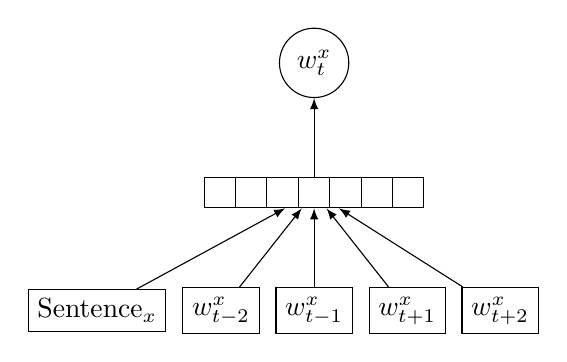
\begin{tikzpicture}[>=latex]
\node[embedding](Sx) {Sentence$_x$};
\node[embedding](W1) [right =0.2cm of Sx] {$w^{x}_{t-2}$};
\node[embedding](W2) [right =0.2cm of W1] {$w^{x}_{t-1}$};
\node[embedding](W4) [right =0.2cm of W2] {$w^{x}_{t+1}$};
\node[embedding](W5) [right =0.2cm of W4] {$w^{x}_{t+2}$};
\node[hidden] (h1) [above =of W2] {} edge[<-] (Sx)edge[<-] (W1)edge[<-] (W2)edge[<-] (W4)edge[<-] (W5);
\node[index] (W3) [above =of h1] {$w^{x}_{t}$} edge [<-] (h1);
\end{tikzpicture}

\caption{PV-DM}
\label{fig:p2v-DM}
\end{subfigure}
\begin{subfigure}{.45\textwidth}\center
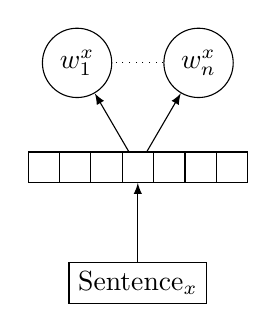
\begin{tikzpicture}[>=latex] 
\node[embedding] (Sx) {Sentence$_x$};
\node[hidden] (h1)[above=of Sx]{} edge [<-] (Sx);
\node (ghost1) [above=of h1] {};
\node[index] (W1) [left =.2 cm of ghost1] {$w^{x}_1$} edge [<-] (h1);
\node[index] (Wn) [right =.2cm of ghost1] {$w^{x}_n$}edge [<-] (h1) edge [ dotted ] (W1);
\end{tikzpicture}
\caption{PV-DBOW}
\label{fig:p2v-DBOW}
\end{subfigure}
\caption{\texttt{paragraph2vec} models}
\end{figure*}

In the DBOW model, no word embeddings are trained. Rather, the sentence embedding is trained by trying to predict the indexes of all words that occur in the sentence (see figure~\ref{fig:p2v-DBOW}).





\subsection{Embeddings for parallel sentences}


This paragraph representation could also be used for encouraging similarity between two bitext sentences.
In our novel approach, we will run the algorithm from \cite{Le2014}, but using the same paragraph vector when training word vectors from parallel sentences.
% is dat genoeg? of moet er iets bij over waarom we denken dat de alignments dan niet nodig zijn?
The sentence representation therefore acts as a way to relate the word spaces in both languages, without using word alignments.
% The method is general enough to allow training on more than two sentences. It also encodes more information in the vector than just bag-of-word-vector based models like Herman & Blunsum
We hope this will create a word vector space that is trainable on both monolingual and parallel data, allowing for the mitigation of sparsity in all languages.

% List of different models within this approach as discussed with Philip
We will explore at least two training methods:
\begin{itemize}
\item 
	Sequentially training all sentence pairs. As a paragraph id, we use a single identifier for every sentence pair in the bitext.
	This is equivalent to concatenating the parallel sentences and training from the context windows that do not bridge the sentence boundary.
\item 
	A two-step process:
	First creating paragraph representations for each sentence pair from a fully trained monolingual model. The information from the words in the first language will create a representation for the sentence.
	Then, we fix the sentence representations and train the word spaces in each language using these vectors.
	These sentence vectors will influence the learning of word embeddings in the other languages.
	The error gradient for the sentence vector can either be distributed over the words or be discarded.
\end{itemize}



The model is depicted in figure~\ref{f:bilingual_dbow}
From the embedding of a single parallel sentence representation, the network tries to predict all words that occur in the sentence either language. Note that no word embeddings are trained, only word indexes are predicted from the sentence embedding. The error is propagated back to train the sentence embeddings.


\begin{figure}

\center
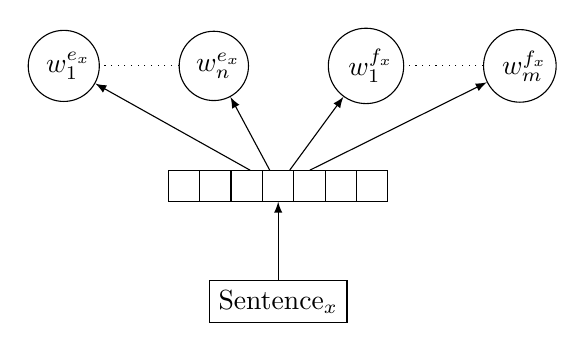
\begin{tikzpicture}[>=latex] 
\node[embedding] (Sx) {Sentence$_x$};
\node[hidden] (h1)[above=of Sx]{} edge [<-] (Sx);
\node[index] (We1) [above left =of h1] {$w^{e_x}_1$} edge [<-] (h1);
\node[index] (Wen) [right =of We1] {$w^{e_x}_n$}edge [<-] (h1) edge [ dotted ] (We1);
\node[index] (Wf1) [right =of Wen] {$w^{f_x}_1$}edge [<-] (h1) ;
\node[index] (Wfm) [right =of Wf1] {$w^{f_x}_m$}edge [<-] (h1) edge [ dotted ] (Wf1);
\end{tikzpicture}
\caption{Bilingual PV-DBOW}
\label{f:bilingual_dbow}
\end{figure}




%Dit niet hier rapporteren?:
Another training procedure relies on the previous experiments. It is based on the distributed memory training from paragraph2vec and  is illustrated in figure~\ref{f:bilingual-dm}. 
The sentence embeddings that resulted from the dbow training were used and kept fixed. The word word embeddings from the previous experiment to initialize the multilingual DM setting. The idea is to further refine the word embeddings using a smaller context. However, the training occurs independently for both languages and the commonality of the semantic space relies solely on the sentence embeddings.

\begin{figure*}

\center
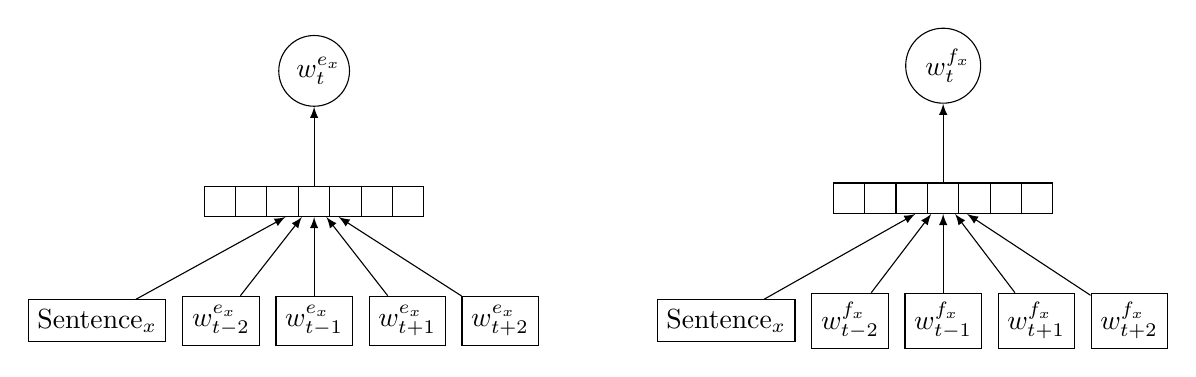
\begin{tikzpicture}[>=latex]
\node[embedding](Sx) {Sentence$_x$};
\node[embedding](We1) [right =0.2cm of Sx] {$w^{e_x}_{t-2}$};
\node[embedding](We2) [right =0.2cm of We1] {$w^{e_x}_{t-1}$};
\node[embedding](We4) [right =0.2cm of We2] {$w^{e_x}_{t+1}$};
\node[embedding](We5) [right =0.2cm of We4] {$w^{e_x}_{t+2}$};
\node[hidden] (h1) [above =of We2] {} edge[<-] (Sx)edge[<-] (We1)edge[<-] (We2)edge[<-] (We4)edge[<-] (We5);
\node[index] (We3) [above =of h1] {$w^{e_x}_{t}$} edge [<-] (h1);

\node[embedding](Sx2) [right=1.5cm of We5]{Sentence$_x$};
\node[embedding](Wf1) [right =0.2cm of Sx2] {$w^{f_x}_{t-2}$};
\node[embedding](Wf2) [right =0.2cm of Wf1] {$w^{f_x}_{t-1}$};
\node[embedding](Wf4) [right =0.2cm of Wf2] {$w^{f_x}_{t+1}$};
\node[embedding](Wf5) [right =0.2cm of Wf4] {$w^{f_x}_{t+2}$};
\node[hidden] (h2) [above =of Wf2] {} edge[<-] (Sx2)edge[<-] (Wf1)edge[<-] (Wf2)edge[<-] (Wf4)edge[<-] (Wf5);
\node[index] (Wf3) [above =of h2] {$w^{f_x}_{t}$} edge [<-] (h2);
\end{tikzpicture}

\caption{Bilingual PV-DM}
\label{f:bilingual-dm}
\end{figure*}


\section{Obtaining multilingual word embeddings}\label{s:wordEmbeddings}

% DM doesn't work
% 
% 

\subsection{Words from PV-DM}
Our first approach to obtaining joint multilingual word embeddings was based on using the word embeddings from the multilingual \texttt{PV-DM}.
However, the error signal that is used to train the word representations does not lend itself for learning a joint multilingual word vector space.
The model is predicting either words in one language or words in the other language, but never both.
This way, the model the model is inadvertently trained to distinguish between the languages.
If both languages had similar embeddings, the model would make prediction errors by predicting the word index for the translation of the target as well.
Therefore, the error signal makes the model distinguish between both languages.

%NB de woordrepresentaties per taal lijken wel goed te zijn
The model does learn sensible word embeddings in both languages independently.
The word embeddings are located near related words in their own language, and far away from embeddings from the other language.

Additionally, if the languages used the features in the same way, subtracting a word from its literal translation could result in a `translation vector'.
This vector could then be added to words in one language to find their counterpart in the other.
However, it seems to be impossible to construct such a vector with this model. 
In this approach the vector dimensions therefore encode different information for both languages and also the sentences.


% % List of different models within this approach as discussed with Philip
% We will explore at least two training methods:
% \begin{itemize}
% \item 
% 	Sequentially training all sentence pairs. As a paragraph id, we use a single identifier for every sentence pair in the bitext.
% 	This is equivalent to concatenating the parallel sentences and training from the context windows that do not bridge the sentence boundary.
% \item 
% 	A two-step process:
% 	First creating paragraph representations for each sentence pair from a fully trained monolingual model. The information from the words in the first language will create a representation for the sentence.
% 	Then, we fix the sentence representations and train the word spaces in each language using these vectors.
% 	These sentence vectors will influence the learning of word embeddings in the other languages.
% 	The error gradient for the sentence vector can either be distributed over the words or be discarded.
% \end{itemize}

% Another training procedure relies on the previous experiments.
% It is based on the Distributed Memory training from paragraph2vec. % and  is illustrated in figure~\ref{f:bilingual-dm}. 
The second approach was to use two separate \texttt{PV-DM} models and strong initialization of the paragraph vectors.
Both models shared the parallel sentence representations, but they independently predicted words from contexts in either language.

For initialization, the sentence embeddings that resulted from the dbow training were used and kept fixed.
The word vectors were initialized to be as near as possible to the embeddings of the sentences that those words appear in.
We therefore initialized every word vector as the average of all sentence embeddings that it occurs in.
% We used the word embeddings from the previous experiment to initialize the multilingual DM setting with two separate models.
The idea was to then further refine the word embeddings using a smaller context in the two \texttt{PV-DM} models.
However, the training occurs independently for both languages and the commonality of the semantic space relies solely on the sentence embeddings.
It was not possible to construct a joint bilingual vector space in this way.


% DBOW does work
% 



\subsection{Words as sentence averages}

However, the word initialization discussed above is interesting in its own right.
Inspired by the bag-of-words additive interpretation of composition, we flip the model upside down.
Instead of assuming that a sentence representation is the average of its word embeddings, we assume a word embedding is the average of the sentences it occurs in.
This way, a word embedding is as close as possible to the representations of all sentences in which it is used.
Word embeddings are thus computed with the following equation:

\begin{equation*}
[\![ w ]\!] =\frac{1}{freq(w,D)}\sum_{s\in D}freq(w,s) [\![ s ]\!]
\end{equation*}

This means the word embeddings are not trained on any information about their direct context.
As with \cite{hermann2013multilingual} and \cite{SarathChandar2014autoencoder}, we assume a bag-of-words sentence representation and train word embeddings from their sentence co-occurrence.

We were unable to convert these word embeddings from sentence co-occurrence into word embeddings from local co-occurrence using the multilingual \texttt{PV-DM} model.
This shows that there is a fundamental difference between the two types of word embeddings.
Word embeddings from sentence co-occurrence reflect the topic of the sentence they occur in, while the local co-occurrence word embeddings reflect more information about word usage within sentences.
Without word alignments, there are no parallel word contexts.
Therefore, there must be notion of word alignment in a model that aims to find word embeddings from local co-occurrence.

The two types of word embeddings should also be evaluated differently and used for different tasks.
Word embeddings from sentences are useful for information retrieval, but tasks that involve a finer-grained sense of word meaning benefit more from word embeddings based on local co-occurrence.
Those tasks include Machine Translation and Semantic Parsing.
\section{Evaluation}\label{s:evaluation}
%Reproducing existing work with more languages
%New approach: based on par2vec (2 flavors)


It is not trivial to measure the quality of the multilingual word embeddings. The semantic space should be reliable for each language in isolation, and consistent across languages. 
Even the former is not easy to assess. In \cite{mikolov2013efficient}, an analogy task is introduced to this aim, which we apply to our English word embeddings.

The latter is evaluated on a real-world task of cross-lingual document classification. The models we use rely on bag-of-word representations of sentences, as explained in section~\ref{s:wordEmbeddings}. Therefore, we do not expect a fine-grained semantic analysis of sentences and words but rather capture something like `topicality'. It thus make sense to apply a document classification task, following the evaluation strategy of  \cite{klementiev2012inducing,hermann2014multilingual}.


\subsection{Word analogy task}
To evaluate word embeddings monolingually, we use the word analogy task described in \cite{mikolov2013efficient}.
The task is based on the intuition that a word like \emph{big} is similar to \emph{biggest} in the same sense that \emph{small} is to \emph{smallest}.
The goal of the task is to answer questions that complete such a relationship, such as ``What word is to \emph{small} what \emph{biggest} is to \emph{big}?''
The answer can be found by adding the difference of $[\![\mathit{biggest}]\!]$ and $[\![\mathit{big}]\!]$ to $[\![\mathit{small}]\!]$, and searching the vocabulary to find the nearest embedding.
In practice, this is done by computing $X = [\![\mathit{biggest}]\!] - [\![\mathit{big}]\!]+ [\![\mathit{small}]\!]$ and comparing all word embeddings by cosine distance.
This finds the embedding that is nearest to \emph{biggest} and \emph{small}, but furthest from \emph{big} \cite{Levy2014}.

We use only the English vocabulary for this task, again trained on the sentence embeddings of the first half million lines of the Europarl corpus.
The accuracy scores are also reported for the vectors from \cite{klementiev2012inducing} and a set of vectors trained on a large Google News corpus \cite{mikolov2013efficient}.
The vocabulary of the Google News embeddings was restricted to contain only words that also occur in our set of Europarl-trained embeddings, which makes the number of answered questions comparable.
This vocabulary thus contains the words that occur 5 or more times in the first half million lines of the Europarl corpus.
It covers about half of the questions in the task, while the vocabulary from \cite{klementiev2012inducing}, trained on part of the Reuters corpus, only covers 1\% of the questions. 
Accuracy scores are computed for only the questions that could be answered with the vocabulary.


\subsection{Document classification - RCV}
In \cite{klementiev2012inducing} a cross-lingual document classification task is introduced. The task, that is also used in \cite{hermann2013multilingual}, is based on Reuters corpora, which has topic-annotated documents. The evaluation data is available for English and German documents that belong to a single topic, and thus the gold standard can be represented by a one-hot vector.

A vector representation is obtained for each document in the dataset. In \cite{klementiev2012inducing}, the document vector is the average of the representations of its \emph{tokens}, weighted by $idf$ score. In \cite{hermann2013multilingual}, the document vector is the average of the representations of its \emph{sentences}. We use both approaches, depending on the experimental settings.

As a classifier, we use the implementation of an averaged perceptron algorithm from \cite{klementiev2012inducing}. It is trained to predict classes (topics) from document representations. In the cross-lingual setting, the perceptron is trained for document classification in one language, and tested on data in another resulting in a classification accuracy score. If the semantic space is coherent between languages, performance should not diverge much between monolingual and cross-lingual document classification. 
%Alternatively, \cite{klementiev2012inducing} compares to wordcount features. Translations are done via glossing or machine translation. It is also common to compare to a MT baseline. 

The topics in the RCV evaluation sets belong to four topics: Corporate/Industrial, Economics, Government/Social, and Markets.
For both languages, the documents are split into train sets with 100, 200, 500, 1000, 5000 and 100000 documents, and a test set of around 5000 documents.
As a baseline, we compute chance accuracy for the majority class estimate. For both languages, the majority class was Markets, with around 46.8\% of the documents.

\subsection{TED document classification}
The WIT TED corpus \cite{cettolo2012} contains short documents with transcriptions and translations of TED talks, with topic annotations. The original distribution was aimed at machine translation, but \cite{hermann2014multilingual} propose it for a multilingual document classification task. The major advantage of this task over the previous one, is the availability of documents in many languages. It has documents in English sentence-aligned with other languages, six of which are also in the Europarl data we use for obtaining our data: Spanish, French, German, Italian, Dutch, and Portuguese.

There are fifteen classification labels, i.e. topics, in this set.
%The classification labels in this set are technology, culture, science, global issues, design, business, entertainment, arts, politics, education, art, health, creativity, economics, and biology. 
Note that contrary to the previous task, a document can have more than one topic annotation. A binary classifier is thus trained for each topic, using the same system as before. Performance is reported both as classification accuracy and F1 score. As the chance accuracy for majority class is quite high, since there are only few positive examples per class, F1 is more informative for comparing performance. 

The majority class estimate is not usable as a baseline for F1 performance: as the majority of the documents are labeled negative, precision would be zero and thus F1 too (or, actually, undefined). As an alternative baseline, we compare to a stochastic classifier that predicts `true' with probability $P=pos/total$. The expected number of True Positives is thus $P*pos=P^2*|X|$, the expected False Positives and False Negatives are both $P*(1-P)*|X|$. We can now compute expected F1:

\begin{align*}
F1	&=\frac{2*TP}{2*TP+FN+FP}\\
			&=\frac{2*P^2*|X|}{2*P^2*|X|+2((1-P)*P*|X|)}\\
			&=P
\end{align*} Therefore, we use the ratio of positive examples as a baseline for the performance on TED data.






%In \cite{mikolov2013exploiting}, the evaluation is performed on a test set of gold-standard word translations, again from Google Translate. The word representation in the source language is transformed using $W$, and a ranked list of the nearest words in the target language is the output. The precision at ranks 1 and 5 is reported. 
% Gaan we dat nou ook nog doen of niet?

%For visualizing the vector space, we will project a selection of words onto a plane and highlight semantic relationships.
%We will also visualize rare words and words with high variability across languages.

\section{Experiments and results}\label{s:experiments}
%Reproducing existing work with more languages
%New approach: based on par2vec (2 flavors)


\subsection{Evaluation}
We evaluate our mutlilingual word embeddings on the same real-world task as \cite{klementiev2012inducing} and \cite{hermann2013multilingual}: crosslingual document classification. The task is based on Reuters corpora, which has topic-annotated documents in English, French, German, Italian and Spanish. These languages are also in the Europarl data. Only documents that are assigned a single topic are used.

Each document is represented by the average of the representations of its tokens (in \cite{klementiev2012inducing}), or sentences (in \cite{hermann2013multilingual}).
An averaged version of the perceptron algorithm is trained for document classification in one language, and tested on data in another.

We thus compute classification accuracy to compare the existing approaches described above to each other and to the new models introduced in \ref{s:newApproach}.

%As a baseline, \cite{klementiev2012inducing} compares to wordcount features. Translations are done via glossing or machine translation.





%Alternative:
The WIT TED corpus \cite{cettolo2012} contains short documents with transcriptions and translations of TED talks, with topic annotations. The original distribution was aimed at machine translation, but \cite{hermann2014multilingual} propose it for a multilingual document classification task.


English paired in both directions with other languages, seven of which are also in the Europarl corpus: Spanish, German, Italian, Dutch, Portuguese, Polish, and Romanian.
%Slovenian is not in the Hermann-Blunsom dataset!
% Non-Europarl: Arabic, Russian, Turkish, and Chinese, Farsi, 

The classification labels in this set are technology, culture, science, global issues, design, business, entertainment, arts, politics, education, art, health, creativity, economics, and biology. Note that a document can have more than one topic annotation. 






%In \cite{mikolov2013exploiting}, the evaluation is performed on a test set of gold-standard word translations, again from Google Translate. The word representation in the source language is transformed using $W$, and a ranked list of the nearest words in the target language is the output. The precision at ranks 1 and 5 is reported. 
% Gaan we dat nou ook nog doen of niet?

%For visualizing the vector space, we will project a selection of words onto a plane and highlight semantic relationships.
%We will also visualize rare words and words with high variability across languages.

\section{Discussion and future work}\label{s:discussion}
%- misschien iets over het feit dat Duits moeilijk is, en dat we geen preprocessing doen.
%- mogelijkheid andere modellen voor woorden uit zinnen (gewogen, CVM model erin plakken à la Hermann&Blunsom)
%- Probleem van word senses, en hoe daarvoor parallel data gebruikt kan worden

Our experiments are somewhat tentative, given the scope of this research. We discuss some considerations and directions for more thorough research.

\subsection{Word senses}
Many approaches to word embeddings assume that each word gets mapped to a single embedding. However, words often posses several senses: different meanings that may be more or less related. In order to improve the quality of semantic spaces, these word senses should be taken into account. Parallel data might actually help to induce word senses, since languages can actually have different words where another language uses the same word for different senses.

\subsection{Issues of morpology}
Of course, languages differ in what it means to be a `word'. English has quite simple morphology, while Latin languages often use inflections and German and Dutch have a lot of compound words. Simple tokenization of text may thus not produce equally reliable vocabularies for different languages, and therefore distort performance. A possible solution is to apply stemming or other morphological decomposition. We have not looked into these possibilities, but it would sure be a good idea to take this in consideration in further research on crosslingual embeddings.

\subsection{Models of composition}
In our experiments, we used a bag-of-words representation of the sentences in the training of sentence embeddings. In the estimation of word embeddings, we assume a reversed additive compositional model: we take the word to be the average of all sentences it occurs in. Although we have not investigated this, alternative weighing schemes could be applied. The weight could be based on features of the sentence and the word, to resemble the salience of the word in that sentence.

Aditionally, a lot of research has focused at more pregnant models of composition, ranging from a bigram additive model \cite{hermann2014multilingual} to complex syntactically inspired constitutionality. Given a sentence representation, whether it is trained with {\tt PV-DBOW} or otherwise, any model of composition could in principle be used to obtain word embeddings.
\section{Conclusion}\label{s:conclusion}
%Er is een verschil tussen lokale en zinscorrelatie. Zonder word alignment kun je het eerste niet doen. Wij presenteren een manier om het tweede te doen. We kunnen best goede woord-embeddings maken van zinrepresentaties. Crosslingual met parallele dbow, maar ook monolingual training. Met parallele data kunnen we vervolgens hier word embeddings van maken.el dbow trainen.

We discovered a fundamental difference between the usage of local and global correlation to establish word embeddings. Without aligning words in parallel data, there is no apparent way to introduce local correlation in cross-lingual induction of word embeddings. However, using global (sentence level) correlation, we can create embeddings that are useful for IR-related tasks. We introduced a model to train {\tt PV-DBOW} sentence representations on parallel data in any number of languages. But we also show that we can obtain word embeddings from sentence representations that are trained on another language, as long as there is parallel data available.

\bibliographystyle{acl2014}
\bibliography{bibliography}

\end{document}